% rubber: module beamer
% rubber: module verbatim
% rubber: module xr
% rubber: clean status.vrb
% rubber: setlist arguments -shell-escape
% rubber: depend struct.c
% rubber: depend struct_introspect.c
% rubber: depend long_struct_introspect.c
% rubber: depend ruminate_simple.c
% rubber: depend ruminate_traverse.c
% rubber: depend ruminate_stack.c
% rubber: depend ruminate_memory.c
% rubber: depend ruminate_jansson_uni.c
% rubber: depend ruminate_jansson_bidi.c
%\documentclass[handouts]{beamer}
\documentclass{beamer}
\usepackage{listings}
\usepackage{bibentry}
\usepackage{verbatim}
\usepackage{fancyvrb}
\usepackage{color}
\usepackage{minted}
\usepackage{ulem}
\usepackage{lmodern}
\usepackage[T1]{fontenc}

\setbeamertemplate{navigation symbols}{}

\usemintedstyle{trac}

\lstset{
	language=C,
	showstringspaces=false,
	basicstyle=\ttfamily
}

%\usepackage{pgfpages}
%\pgfpagesuselayout{4 on 1}[letterpaper,border shrink=4mm]
%\setbeamertemplate{footline}[page number]

\title{Introspection via Self Debugging}
\author{\texorpdfstring{Russell Harmon\newline\url{reh5586@cs.rit.edu}}{Russell Harmon}}
\institute {
	Rochester Institute of Technology\newline
	Computer Science\newline
}
\date{December 12, 2013}

\begin{document}
\maketitle

\begin{frame}
	\frametitle{Overview}
	\tableofcontents
\end{frame}

\section{Debuggers}

\begin{frame}
	\frametitle{Debugger}

	\begin{quote}
		... a computer program that is used to test and debug other programs -Wikipedia
	\end{quote}

	\pause

	\begin{itemize}
		\item LLDB - LLVM debugger
		\item GDB - GNU debugger
		\item WinDBG - Windows debugger
		\item DBX - Sun Studio debugger
		\item LDB - Intel debugger
	\end{itemize}
\end{frame}

\begin{frame}
	\frametitle{Debugging Example}

	\inputminted[tabsize=4,linenos]{c}{struct.c}
\end{frame}

\begin{frame}[fragile]
	\frametitle{Debugging Example}

	\begin{Verbatim}[commandchars=\\\{\}]
		(lldb) \textcolor{red}{run}
		* thread #1: tid = 0x1c03, 0x0000000100000f65
		  a.out`main + 21 at struct.c:9, stop reason =
		  EXC_BREAKPOINT (code=EXC_I386_BPT, subcode=0x0)
		    frame #0: 0x0000000100000f65 a.out`main + 21
		    at struct.c:9
		   6      struct foo bar;
		   7      bar.str = "Hello World!";
		   8      asm("int $0x3");
		-> 9    \}
	\end{Verbatim}
\end{frame}

\begin{frame}[fragile]
	\frametitle{Debugging Example}

	\begin{Verbatim}[commandchars=\\\{\}]
		(lldb) run
		* thread #1: tid = 0x1c03, 0x0000000100000f65
		  a.out`main + 21 at struct.c:9, stop reason =
		  EXC_BREAKPOINT (code=EXC_I386_BPT, subcode=0x0)
		    frame #0: 0x0000000100000f65 a.out`main + 21
		    at struct.c:9
		   6      struct foo bar;
		   7      bar.str = "Hello World!";
		   8      asm("int $0x3");
		-> 9    \}
		(lldb) \textcolor{red}{print bar}
		(foo) $0 = \{
		  (char *) str = 0x0000000100000f67 "Hello World!"
		\}
	\end{Verbatim}
\end{frame}

\begin{frame}[fragile]
	\frametitle{Debugging Example}

	\begin{Verbatim}[commandchars=\\\{\}]
		(lldb) print bar
		(\textcolor{red}{foo}) $0 = \{
		  (\textcolor{red}{char *}) str = 0x0000000100000f67 "Hello World!"
		\}
	\end{Verbatim}
	\pause
	\inputminted[tabsize=4,linenos]{c}{struct.c}
\end{frame}

\section{Introspection}

\begin{frame}[fragile]
	%\bibliographystyle{abbrv}
	%\nobibliography{status.bib}

	\frametitle{Introspection}
	\begin{quote}
		... the ability for a program to examine the type or properties of an object
		at runtime. -Wikipedia
	\end{quote}

	\begin{itemize}
		\item Interpreted languages have reflection / introspection.
		\item introspection $\subset$ reflection

		\item {
			\lstset{language=Java}
			Java: \lstinline!this.getClass().getCanonicalName()!
		}

		\item {
			\lstset{language=Ruby}
			Ruby: \lstinline!self.class.name!
		}
	\end{itemize}
\end{frame}

\section{Introspection + Debugging}

\begin{frame}[fragile]
	\frametitle{Introspection + Debugging}

	\inputminted[tabsize=4,linenos]{c}{struct_introspect.c}
	\pause
	\begin{verbatim}
		foo
		char *
	\end{verbatim}
\end{frame}

\begin{frame}[fragile]
	\frametitle{Use Cases}

	\begin{itemize}[<structure@+>]
		\item \mint{c}!abort_with_stacktrace();!
		\item easy data structure traversal
		\item access to third party library internals
	\end{itemize}
\end{frame}

\section{Ruminate}
\subsection{Use}

\begin{frame}
	\frametitle{Ruminate}

	\begin{itemize}[<structure@+>]
		\item Introspective library for C
		\item Data introspection (structs, unions, enums, functions, primitives)
		\item Stack introspection
	\end{itemize}
\end{frame}

\begin{frame}[fragile,shrink]
	\frametitle{Ruminate}
	\framesubtitle{Simple Use}

	\inputminted[tabsize=4,linenos]{c}{ruminate_simple.c}
	\pause
	\begin{verbatim}
		foo
		char *
	\end{verbatim}
\end{frame}

\begin{frame}[fragile]
	\frametitle{Ruminate}
	\framesubtitle{Simple Use}

	A rundown of the ruminate functions used

	\begin{itemize}
		\item \lstinline|ruminate_init| initializes Ruminate
		\item \lstinline|ruminate_get_type| retrieves an \lstinline|RType| representing a
			type
		\item \lstinline|r_type_name| retrieves an \lstinline|RString| containing the
			name of an \lstinline|RType|
		\item \lstinline|r_string_bytes| retrieves a \lstinline|char *| containing the
			value of an \lstinline|RString|
	\end{itemize}
\end{frame}

\begin{frame}
	\frametitle{Ruminate}

	Ok, but that's \emph{really} simple...
\end{frame}

\begin{frame}[fragile,shrink]
	\frametitle{Ruminate}
	\framesubtitle{Type Traversal}

	\inputminted[tabsize=4,linenos]{c}{ruminate_traverse.c}
	\pause
	\begin{verbatim}
		char *
	\end{verbatim}
\end{frame}

\begin{frame}[fragile]
	\frametitle{Ruminate}
	\framesubtitle{Type Traversal}

	Only a few new functions

	\begin{itemize}
		\item \lstinline|r_aggregate_type_member_by_name| gets a member of an
      aggregate type by it's name
		\item \lstinline|r_type_member_type| gets the type of an aggregate member
	\end{itemize}
\end{frame}

\begin{frame}
	\frametitle{Ruminate}
	\framesubtitle{Type Hierarchy}

	\begin{figure}
		\begin{center}
		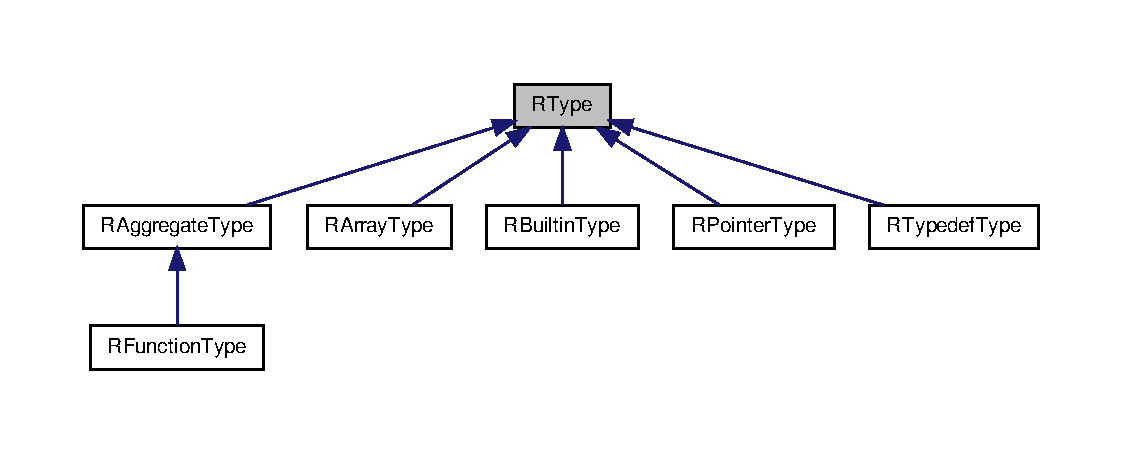
\includegraphics[width=307pt]{struct_r_type__inherit__graph}
		\end{center}
	\end{figure}
\end{frame}

\begin{frame}
	\frametitle{Ruminate}

	Still too simple?

	\pause

	Ok, well there's this
\end{frame}

\begin{frame}[fragile,shrink]
	\frametitle{Ruminate}
	\framesubtitle{Complex Example}

	\inputminted[tabsize=4,linenos=false]{c}{long_struct_introspect.c}
\end{frame}

\begin{frame}
	\frametitle{Ruminate}

	But that's too large to fit.
\end{frame}

\begin{frame}
	\frametitle{Ruminate}

	Oh wait

	\pause

	Lets not forget

	\pause

	You can do stack introspection too
\end{frame}

\begin{frame}[fragile,shrink]
	\frametitle{Ruminate}
	\framesubtitle{Stack Introspection}

	\inputminted[tabsize=4,linenos]{c}{ruminate_stack.c}
	\pause
	\begin{verbatim}
		ruminate_hit_breakpoint
		ruminate_backtrace
		print_backtrace
		bar
		bar
		bar
		foo
		main
		__libc_start_main
	\end{verbatim}
\end{frame}

\begin{frame}[fragile,shrink]
	\frametitle{Ruminate}
	\framesubtitle{Typed Memory Allocator}

	Building on this, you can do typed dynamic memory allocation.

	\pause

	\inputminted[tabsize=4,linenos]{c}{ruminate_memory.c}

	\begin{Verbatim}
		(char *) "Hello World!"
	\end{Verbatim}
\end{frame}

\begin{frame}[fragile,shrink]
	\frametitle{Ruminate}
	\framesubtitle{JSON}

	and do transparent json conversion

	\pause

	both unidirectionally

	\inputminted[tabsize=4,linenos]{c}{ruminate_jansson_uni.c}

	\begin{Verbatim}
		{"i": 1, "e": 1}
	\end{Verbatim}
\end{frame}

\begin{frame}[fragile,shrink]
	\frametitle{Ruminate}
	\framesubtitle{JSON}

	and bidirectionally

	\inputminted[tabsize=4,linenos]{c}{ruminate_jansson_bidi.c}

	\begin{Verbatim}
		{"value": {"i": 1, "e": 1}, "type": "MyStruct"}
	\end{Verbatim}
\end{frame}

\subsection{Internals}

\begin{frame}
	\frametitle{Implementation}

	Lets dive in
\end{frame}

\begin{frame}[fragile]
	\frametitle{Implementation}
	\framesubtitle{RType}

	\begin{minted}[tabsize=4,linenos]{cpp}
		struct RType {
		    RTypeId id;
		    gint refcnt;
		    RString *name;
		    RuminateBackend::TypePrx type;
		    RuminateBackend::TypeId type_id;
		    struct {
		        size_t value;
		        bool initialized;
		    } size;
		};
	\end{minted}

	\pause

	Aside from caching, \lstinline|RType| is just a proxy backed by
	\lstinline|RuminateBackend::TypePrx|
\end{frame}

\begin{frame}[fragile,shrink]
	\frametitle{RPC Contract}

	\begin{itemize}
		\item Simple, minimal RPC interface
		\item Built off the \lstinline|Type| interface
		\item Should be simple enough to port to other debuggers
	\end{itemize}

	\pause

	\begin{minted}[tabsize=4,linenos]{java}
		interface Type {
		  TypeId getId();
		  Type *getPointeeType();
		  Type *getPointerType();
		  Type *getCanonicalType();
		  Type *getReturnType();
		  Type *getArrayMemberType();
		  idempotent long getArrayLength();
		  TypeMemberList getMembers( optional(1) long tid );
		  string getName();
		  idempotent long getSize();
		  idempotent bool isSigned();
		  idempotent bool isUnsigned();
		};
	\end{minted}
\end{frame}

\begin{frame}
	\frametitle{Implementation}
	\framesubtitle{RType}
	\lstinline|RType| and it's decendants:

	\begin{itemize}
		\item type safe
		\item caching
		\item reference counted
		\item wrapper around \lstinline|Type|
	\end{itemize}
\end{frame}

\begin{frame}
	\frametitle{Implementation}
	\framesubtitle{Debugger Server}

	Manipulate LLDB to implement the RPC contract

	\pause

	Some interesting bits
	\begin{itemize}
		\item Enums
		\item Signals
		\item Arrays
	\end{itemize}
\end{frame}

\begin{frame}
	\frametitle{Implementation}
	\framesubtitle{LLDB}

	\begin{itemize}
		\item DWARF
		\item ELF, Mach-O
		\item Name demangling
		\item Stack traversal
	\end{itemize}
\end{frame}

\begin{frame}[fragile]
	\frametitle{Implementation}
	\framesubtitle{Enums}

	LLDB's public API did not support enum introspection. Support was added.

	\pause

	Enum members are interesting

	\pause

	the only \emph{type} in C whose value is part of the type

	\begin{minted}{c}
		enum MyEnum {
		    MY_ENUM_1,
		    MY_ENUM_2
		};
	\end{minted}
\end{frame}

\begin{frame}
	\frametitle{Implementation}
	\framesubtitle{Signals}

	\begin{quote}
		While being traced, the tracee will stop each time a signal is delivered
		-ptrace(2)
	\end{quote}

	LLDB default behavior is to stop on (most) signals and wait for user input...

	\pause

	there is no user
\end{frame}

\begin{frame}
	\frametitle{Implementation}
	\framesubtitle{Signal Deadlock}

	If a signal occurrs, LLDB will wait for the debugee to provide instructions.
	The debugee will remain stopped.

	\pause

	change LLDB's signal disposition to ignore signals

	No support for this in LLDB. Support was added.
\end{frame}

\begin{frame}[fragile]
	\frametitle{Implementation}
	\framesubtitle{Arrays}

	LLDB does not model arrays in it's pure type representation.

	\pause

	Arrays are accessed by \emph{value} only.

	\pause

	\begin{minted}{c}
		char a[sizeof((*((int (*)[4]) NULL))[0])];
		__typeof__(&a) ap = &a;
		(int (*)[4]) ap
	\end{minted}
\end{frame}

\begin{frame}
	\frametitle{Implementation}
	\framesubtitle{Typed Memory}

	Typed memory is implemented by padding the beginning of allocated memory with
	a pointer to the type.


\end{frame}

\begin{frame}[fragile,shrink]
	\frametitle{Implementation}
	\framesubtitle{JSON}

	Conversion to JSON is simple

	\begin{Verbatim}
		if the type is a struct
		  generate a JSON object
		  for each subtype
		    recurse
		else if the type is an enum
		  generate a JSON integer
		else if the type is an array
		  generate a JSON array
		  recurse
		else if the type is a pointer
		  recurse using the dereferenced pointer
		else
		  generate a JSON primitive
	\end{Verbatim}

	Note that unions and strings are not handled.
\end{frame}

\begin{frame}[fragile,shrink]
	\frametitle{Implementation}
	\framesubtitle{JSON}

	Conversion from json is similar

	\begin{Verbatim}
		retrieve the name of the type from the top-level json object
		lookup the type in the current program
		allocate typed memory
		proc repeat
		  if the type is a struct
		    retrieve the JSON object representing this value
		    for each subtype
		      call repeat
		  else if the type is an enum
		    insert the value of the JSON int
		  else if the type is an array
		    retrieve the JSON array representing this value
		    call repeat
		  else if the type is a pointer
		    allocate typed memory
		    call repeat
		  else
		    insert the value from the JSON primitive
	\end{Verbatim}
\end{frame}

\section{Limitations}

\begin{frame}
	\frametitle{Limitations}

	\begin{itemize}
		\item strings are not detectable
		\item the current type of a union is not detectable
		\item slow
		\item debugging symbols are required
	\end{itemize}
\end{frame}

\begin{frame}
	\frametitle{Limitations}
	\framesubtitle{Strings}

	strings are not detectable

	\pause

	In C, a string has type \lstinline|char *|.
	That is, it's type is "pointer to byte".

	With no additional information it is \emph{unknowable} if this
	\lstinline|char *| type is
	
	\begin{itemize}
		\item a valid \lstinline|NULL| terminated string
		\item a pointer to a single character
		\item a pointer to multiple characters which is non \lstinline|NULL| terminated
		\item a pointer to one or more bytes which are not valid characters in the
			current encoding
	\end{itemize}
\end{frame}

\begin{frame}[fragile]
	\frametitle{Limitations}
	\framesubtitle{Unions}

	The current type of a union is not detectable

	\pause

	\begin{minted}[linenos]{c}
		union foo { int a; char b; }
		int main( int argc ) {
		    union foo f;
		    if( argc > 2 ) {
		        f.a = 1;
		    } else {
		        f.b = 'c';
		    }
		    // !!
		}
	\end{minted}

	\begin{itemize}
		\item The compiler cannot know the type of \lstinline|f| at line 9 due to the
			indeterminate nature of \lstinline|argc|
		\item The debugger cannot know the type of \lstinline|f| at line 9 because
			DWARF does not (and cannot) contain enough information for the debugger to
			determine the current type of \lstinline|f|
	\end{itemize}
\end{frame}

\begin{frame}[fragile,shrink]
	\frametitle{Limitations}
	\framesubtitle{Slow}

	Ruminate imposes significant overhead.

	\inputminted[tabsize=4]{c}{ruminate_memory.c}

	Takes ~1.6 seconds to run.
\end{frame}

\begin{frame}
	\frametitle{Limitations}
	\framesubtitle{Debugging Symbols}

	Debugging symbols are required

	\pause

	Not a limitation

	\pause

	DWARF debugging symbols are made up of two components:
	\begin{itemize}
		\item line number information
		\item type information
	\end{itemize}
	all of which is available in every other language that has introspection.
	
	\pause

	Debugging symbols are only required in modules being introspected.
\end{frame}

\section{Future Work}

\begin{frame}
	\frametitle{Future Work}

	slow is a problem

	\pause

	eliminate the debugger controller

	\pause

	embed the debugger inside the debugee

	\pause

	how?
\end{frame}

\begin{frame}
	\frametitle{Future Work}

	what makes a debugger?

	\pause

	\begin{itemize}
		\item remote process controller
		\item remote memory inspector
		\item executable parser (ELF, Mach-O, etc)
		\item symbol parser
		\item stack traverser
	\end{itemize}
\end{frame}

\begin{frame}
	\frametitle{Future Work}

	what does Ruminate need?

	\pause

	\begin{itemize}
		\item \sout{remote process controller}
		\item \sout{remote memory inspector}
		\item executable parser (ELF, Mach-O, etc)
		\item symbol parser
		\item stack traverser
	\end{itemize}
\end{frame}

\begin{frame}
	\frametitle{Future Work}

	how?

	\pause

	split LLDB's core into several components
	\begin{itemize}
		\item symbol parser
		\item stack traverser
	\end{itemize}
	useful for more than just Ruminate
\end{frame}

\begin{frame}
	\begin{centering}
		Thanks
	\end{centering}
\end{frame}

%\begin{frame}
%	\frametitle{Prior Research}
%
%	None!
%
%	{
%		\footnotesize
%		\begin{itemize}
%			\item \bibentry{Marinescu:2011:ETR:2063509.2063511}
%			\item \bibentry{Frampton:2009:DMH:1508293.1508305}
%			\item \bibentry{Carbone:2009:MKO:1653662.1653729}
%		\end{itemize}
%	}
%\end{frame}
%
%\begin{frame}
%	\frametitle{End}
%
%	Questions?
%\end{frame}

\end{document}
% vim:noet ts=2 sts=2 sw=2 tw=80
